\documentclass[12pt,twoside, a4paper, twocolumn]{article}
\usepackage[utf8]{inputenc}
\usepackage[brazil]{babel}
\usepackage[margin = 0.5in]{geometry}
\usepackage{amsmath}
\usepackage{amsthm}
\usepackage{amssymb}
\usepackage{amsthm}
\usepackage{setspace}
\usepackage[americanvoltages,fulldiodes,siunitx]{circuitikz}
\usepackage{lipsum}
\usepackage{pgfplots}
\usepackage{ifthen}
\usepackage{adjustbox}
\usepackage[section]{placeins}
\usepackage{hyperref}
\usepackage{graphicx}
\usepackage{amsmath}
\usepackage{amsthm}
\usepackage{amssymb}
\usepackage{amsthm}
\usepackage{setspace}
\usepackage[americanvoltages,fulldiodes,siunitx]{circuitikz}
\usepackage{lipsum}
\usepackage{pgfplots}
\usepackage{ifthen}
\usepackage{adjustbox}
\usepackage[section]{placeins}
\usepackage{hyperref}
\usepackage{graphicx}
\usepackage{adjustbox}
 
\pgfplotsset{compat=newest}
 
\graphicspath{ {./images/} }
 
%  #1 color - optional #2 x_0 #3 y_0 #4 x_f #5 y_f #6 name - optional  #7 true if adding lines to axis
 
\newcommand{\drawvector} [9] [color=cyan] {
   \draw[line width=1.5pt,#1,-stealth](axis cs: #2, #3)--(axis cs: #4, #5) node[anchor=south west]{$#6$};
 
  
 
\ifthenelse{\equal{#7}{true}}{
   \draw[line width=1pt,#1, dashed](axis cs: #4, #5)--(axis cs: #4, 0) node[anchor= north west]{$#8$};
   \draw[line width=1pt,#1, dashed](axis cs: #4, #5)--(axis cs: 0, #5) node[anchor=south east]{$#9$};
   }
   {}
}
 
\newcommand\deriv[2]{\frac{\mathrm d #1}{\mathrm d #2}}
 
 
\title{Primeiro Relatório de Medidas Eletromagneticas}
\author{Gabriel Soares \\ Henrique da Silva}
\date{\today}
\pgfplotsset{width = 10cm, compat = 1.9}
 
 
\begin{document}
\maketitle
\pagenumbering{gobble}
\newpage
%pagenumbering{roman}
\tableofcontents
\newpage



\section{Introdução}


\subparagraph*{Neste relatório, vamos discutir o comportamento de um multimetro, e como ele induz erros para certas bandas de frequencia e o por que.}

\subparagraph*{Todos arquivos utilizados para criar este relatorio, e o relatorio em si estão em:  \url{https://github.com/Shapis/ufpe_ee/tree/main/5th semester/lab circuitos}}




\subsection{Analise preliminar}
\subparagraph*{}


\subparagraph*{Analisaremos a maneira que o multimetro mede tensoes.}

\subparagraph*{Especificamente mediremos uma tensao conhecida de $5\,V_{pp}$, e analisaremos o erro absoluto da medicao em funcao da frequencia provinda do gerador de sinais.}

\subparagraph*{Faremos isto para dois tipos de onda de entrada, senoidal e serra.}

\section{Resultados esperados}

\subsection{Onda senoidal}

\subparagraph*{Para a onda  senoidal esperamos que o erro seja mais alto para frequencias baixas, e para frequencais altas.}

\subparagraph*{Isto ocorre porque o multimetro tem uma banda de confianca, quando nos afastamos desta banda de confianca, perdemos a certeza nas medidas.}

\subsection{Onda dente de serra}

\subparagraph*{Neste caso temos que lembrar que podemos decompor a onda em senoidais por serie de Fourier. E como vimos anteriormente as decomposicoes que tiverem frequencia alta ou baixa serao problematicas.}

\subparagraph*{Mas esperamos que os erros sejam mais distribuidos ao longo da banda inteira que testarmos.}

\section{Medicoes no Laboratorio}

\subparagraph*{Vamos utilizar o osciloscopio para medir uma tensao de saida  conhecida do osciloscopio, esta de $5 V_{pp}$. E registraremos o erro absoluto e relativo entre nossas medidas e a esperada de  $5 V_{pp}$.}

\subsection{Tabela de medicoes}

\begin{center}
    \begin{tabular}{ |c|c|c| }
        \hline
        Freq (Hz) & Erro (V) & Erro  \\
        10        & 0.1818   & 3.58  \\
        15        & 0.1267   & 2.50  \\
        60        & 0.0930   & 1.83  \\
        120       & 0.0916   & 1.80  \\
        300       & 0.0913   & 1.80  \\
        600       & 0.0924   & 1.82  \\
        1000      & 0.0941   & 1.85  \\
        10000     & 0.1139   & 2.25  \\
        20000     & 0.1388   & 2.74  \\
        30000     & 0.1219   & 2.40  \\
        40000     & 0.1114   & 2.19  \\
        50000     & 0.0766   & 1.51  \\
        60000     & 0.0373   & 0.73  \\
        70000     & 0.0050   & 0.10  \\
        80000     & 0.0162   & 0.32  \\
        90000     & 0.0247   & 0.49  \\
        100000    & 0.0213   & 0.42  \\
        110000    & 0.0068   & 0.13  \\
        120000    & 0.0172   & 0.34  \\
        130000    & 0.0497   & 0.98  \\
        140000    & 0.0893   & 1.76  \\
        150000    & 0.1349   & 2.66  \\
        160000    & 0.1858   & 3.66  \\
        170000    & 0.2401   & 4.73  \\
        180000    & 0.2995   & 5.90  \\
        190000    & 0.3606   & 7.10  \\
        200000    & 0.4253   & 8.38  \\
        250000    & 0.7718   & 15.21 \\
        300000    & 1.1342   & 22.35 \\
        330000    & 1.1342   & 26.11 \\
        \hline
    \end{tabular}
\end{center}

\subsection{Graficos dos dados}

\subsubsection{Erro absoluto por frequencia}

\begin{adjustbox}{scale=0.30}
    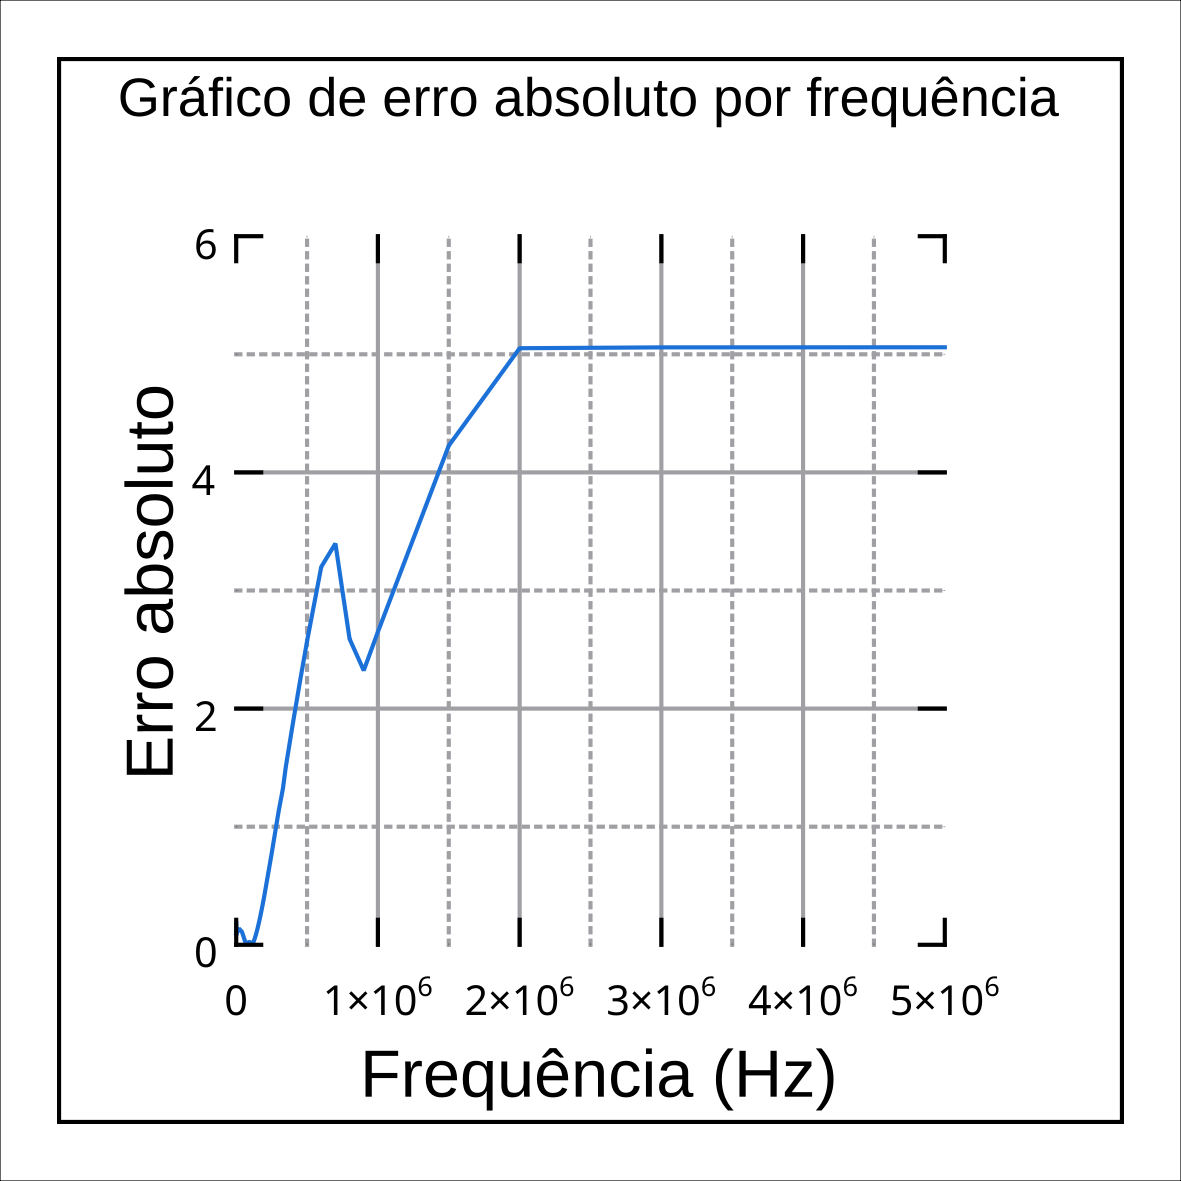
\includegraphics{Grafico1.png}
\end{adjustbox}

\subsubsection{Erro percentual por frequencia}

\begin{adjustbox}{scale=0.30}
    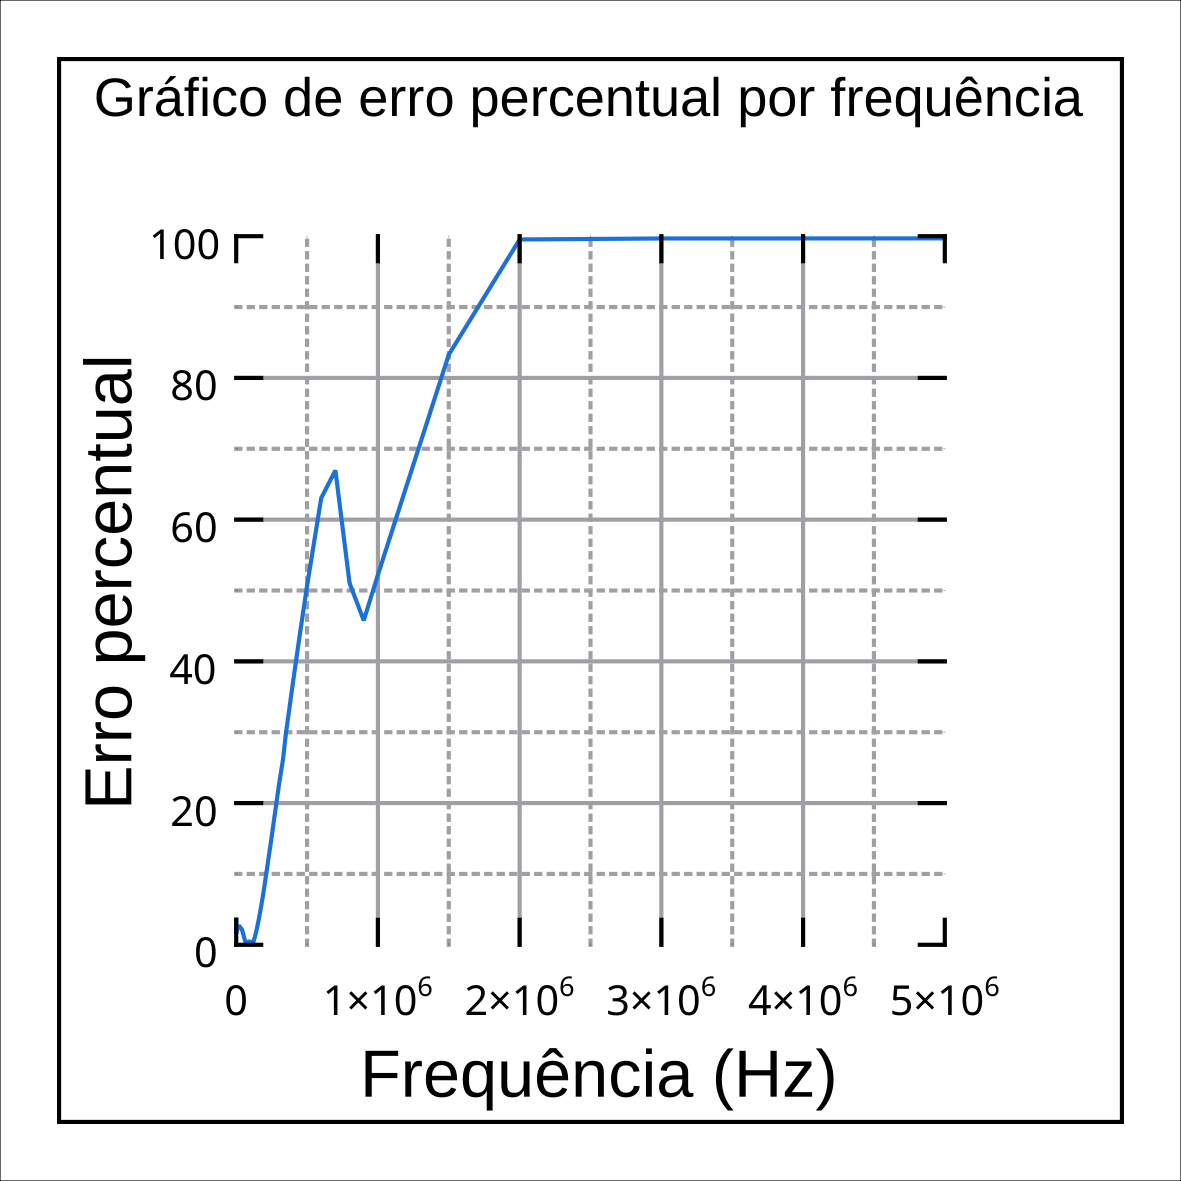
\includegraphics{Grafico2.png}
\end{adjustbox}

\subsection{Analise da onda dente de serra}

\subparagraph*{Quando analisamos este tipo de onda vimos erros distribuidos ao longo de toda banda de testes.}

\subparagraph*{Isto ocorreu por que a funcao dente de serra pode ser decomposta em senoides, e estas multiplas senoides, obedecerem o erro de acordo com os graficos acima na secao \emph{3.2}.}


\subparagraph*{Logo as senoides decompostas de alta frequencia e baixa nos deram um certo erro consideravel, porem distribuido em toda banda  de testes.}

\newpage
\section{Conclusoes}

\subparagraph*{Vemos que o multimetro tem bastante confianca em uma faixa intermediaria, mas fora desta a confianca eh reduzida significantemente.}

\subparagraph*{Precisamos levar em consideracao tambem o formato da onda de entrada e sua decomposicao por serie de Fourier.}

\subparagraph*{Outro ponto que nao abordamos nesta pratica foi o aspecto da calibracao do multimetro. Esta pode afetar tanto a banda de frequencia de confianca quanto a confianca em todos pontos da banda.}


\end{document}